% 原文 pp.202–207（印刷 pp.1320–1325）
% 承接第 14 讲第 1 部分：本文件自 §14.3.3 起，故不写 \section

% ===== 原文 p.202 =====

\subsection{局域算符的 $Q$-上同调与态的 $Q$-上同调的比较}
% 原文 §14.3.3：Comparison of $Q$-cohomology of local operators and $Q$-cohomology of states

我们已经见过两类 $Q$-上同调（$Q$-cohomology）：第一类涉及局域算符（local operator），给出的是手征环（chiral ring）；第二类涉及圆周上的态（state）。现在我们来在这两类 $Q$-上同调之间构造一个映射。我们考虑一个带点 $p$ 的圆盘或半球（hemisphere），如图所示。

\begin{figure}[htbp]
  \centering
  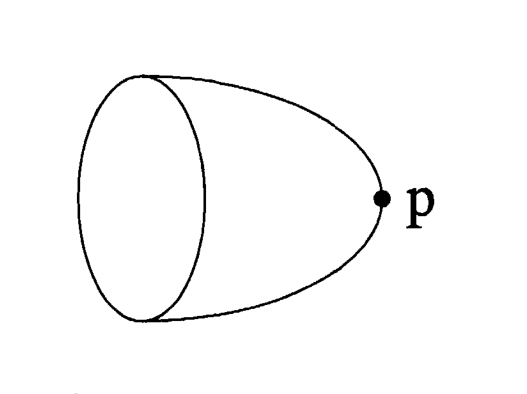
\includegraphics[width=0.40\textwidth]{figs/fig_p202_1.png}
  \caption{带标记点 $p$ 的圆盘（半球）：左侧椭圆表示其边界圆周，$p$ 是内部一点（图中以实心点标出）。在此区域上以给定的边界值作路径积分，便得到从 $p$ 处局域算符到边界场 Hilbert 空间的映射 $\psi$。（原文 Figure 1，p.202）}
  \label{fig:p202-1}
\end{figure}

设 $O$ 是 $p$ 处的一个局域算符。在给定边界值的条件下，对半球上所有场构型作路径积分会给出一个数；当边界值变动时，这个数就成为边界上场的函数。此函数是把边界上的场量子化所得的 Hilbert 空间 $\mathcal H$ 中的一个元素。于是这就给出从 $p$ 处局域算符到 $\mathcal H$ 的一个映射。该映射与 $Q$ 的作用对易，因为路径积分是 $Q$ 不变的；因此它诱导出从局域算符的 $Q$-上同调（即手征环）到圆周上态的 $Q$-上同调 $H^*(Q)$ 的一个映射：
\[
  \psi:(\text{手征环})\longrightarrow H^*(Q).
\]

若 $\mathcal H$ 上 $Q$ 的谱（至少在零点附近）是离散的，则 $\psi$ 是同构。

若 $J_L$ 与 $J_R$ 经典地都是 $R$ 对称性，则手征环与 $\ker H$ 都被这两个对称性赋予双分级（bigrading）。在扭曲理论中，通常分级会出现反常（anomaly），其大小正比于 Riemann 面的 Euler 示性数（对半球而言等于 $1$）。在这种情况下，映射 $\psi$ 把双分级平移
\[
  \psi:H^{p,q}(Q)\longrightarrow \ker H^{p\pm k,\,q\pm k},
\]
其中 $k$ 是反常大小的一个度量。（符号取决于我们所选的是四种扭曲理论中的哪一种。）注意双分级未必按整数分级，而只按有理数分级；这些有理数的分母整除真正作用于理论之上的那个 $U(1)\times U(1)$ 的覆盖的阶。

% [Tutor Note: 此处的 ``$\ker H$'' 指 Hamilton 量 $H$ 的核，而不是「某个映射 $H$ 的核」。在扭曲理论中 $Q$ 是 BRST 型算符，且 $H=\{Q,Q^\dagger\}$，故 $\ker H\subset\ker Q$，而 Hodge 理论给出分解 $\ker Q=\ker H\oplus\operatorname{im}Q$；于是 $\ker H$ 恰是 $Q$-上同调 $H^*(Q)$ 的调和代表空间。作者之所以把两者当成同一对象、并在 $\ker H^{p\pm k,q\pm k}$ 上直接继承双分级，正是用了这一等同。若把它误读成 $H^*(Q)$ 之外的另一个空间，p.204 脚注 2 中「取 $\chi=1$ 时该反常正好产生 §14.3 末尾所说的双分级平移」这句话就无法对上。另需注意：平移量 $k$ 与 $\chi(\Sigma)$ 成正比，而 $\chi(\text{半球})=1$，所以这个例子只是把 $k$ 定标到 $\chi=1$；p.204 的规范理论例子会给出 $k$ 正比于 $\dim G$（而不是每个场贡献 $1$），这才是核对符号与量纲的现成判据。]

\subsection{一个规范理论的例子}
% 原文 §14.4：A Gauge Theory Example

我们取的第一个例子是简单 Lie 群 $G$ 的规范理论。我们从四维的 $\mathcal N=1$ 超对称规范理论出发，做维数约化（dimensional reduction），得到二维的 $\mathcal N=2$ 超对称理论。正如我们在「超习题」（Superhomework）中所见，基本的场强（field strength）是场
\[
  \Sigma=\{\overline{\mathcal D}_+,\mathcal D_-\},
\]
它是取值于主丛（principal bundle）的伴随丛（adjoint bundle）的扭曲手征超场（twisted chiral superfield）。我们使用展开
\[
  \Sigma=\sigma+\cdots+\bar\theta^+\theta^-(F+iD).
\]

% ===== 原文 p.203 =====

玻色场是联络 $A_\mu$ 以及 $\sigma,\bar\sigma$。回忆四维空间上的联络为
\[
  A^{(4)}=\sum_{\mu=0}^{1}A_\mu\,dy^\mu+\sigma(dy^2-i\,dy^3)+\bar\sigma(dy^2+i\,dy^3).
\]
两个 $R$ 对称性是
\[
  J_A=J_L-J_R;\qquad J_V=J_L+J_R.
\]
前者由 $(y^2,y^3)$ 平面内的转动诱导，后者来自四维中的手征 $U(1)$ $R$ 对称性。（该对称性在四维中是反常的，但在二维中不反常——见「超习题」。）现在我们按 $J_V$ 做扭曲，于是 $SO(2)'_E$ 由 $K'=K\pm\tfrac12J_V$ 生成。此时 $A_\mu$ 仍是联络 1-形式，而 $\sigma,\bar\sigma$ 成为 0-形式。一般说来，这种扭曲消去了自旋丛（spin bundle），并把自旋丛的截面变成微分形式。于是四个旋量场 $\lambda_\pm,\bar\lambda_\pm$ 被扭曲成一个 0-形式 $\eta=\psi_{(0)}$、一个 1-形式 $\psi=\psi_{(1)}$ 和一个 2-形式 $\chi=\psi_{(2)}$。（这个新理论当然是存在于紧致曲面上的拓扑理论。它并不具备物理模型所要求的全部通常性质！）

在本例中，$J_A$ 是 $(y^2,y^3)$ 空间转动的两倍，其归一化使得 $[J_A,Q]=Q$。Lagrange 量中各传播场（propagating field）的 $J_A$ 次数如下（参看 [I-Supersolutions, §9.2] 末尾）。（提到「传播场」，意思是我们要用运动方程把辅助场 $F+iD$ 表示为其余场的某个表达式；$F$ 被取为 $A$ 的曲率，$D$ 被取为零，因为理论中没有物质场。）

\begin{center}
\begin{tabular}{|c|c|c|c|c|c|}
\hline
$J_A$-degree & $-2$ & $-1$ & $0$ & $1$ & $2$\\
\hline
field & $\bar\sigma$ & $\psi_{(0)},\psi_{(2)}$ & $A_\mu$ & $\psi_{(1)}$ & $\sigma$\\
\hline
\end{tabular}
\end{center}

% [Tutor Note: 这张表最容易出错之处，是把它读成「形式次数」表。$\sigma$ 与 $\bar\sigma$ 都是 0-形式，$J_A$ 次数却分别是 $+2$ 与 $-2$；而 0-形式的 $\eta=\psi_{(0)}$ 与 2-形式的 $\chi=\psi_{(2)}$ 反而都取 $-1$。正确的读法是「$R$ 荷」表：$\sigma$ 是扭曲手征超场的最高分量以外的标量，带 $R$ 荷 $2$；$\psi_{(k)}$ 的 $J_A$ 次数随形式次数 $k$ 递增。一个立刻可做的自洽性检验是用 p.204 的变换律要求 $\delta$ 把 $J_A$ 次数统一抬高 $1$：由 $\delta\bar\sigma=\psi_{(0)}$ 得 $\deg\bar\sigma=-2$，由 $\delta\psi_{(2)}=F_A$ 得 $\deg F_A=0$，由 $\delta\psi_{(1)}=-D_A\sigma$ 得 $\deg\sigma=+2$（因 $D_A$ 不带 $R$ 荷），由 $\delta\psi_{(0)}=[\sigma,\bar\sigma]$ 得 $2+(-2)=0$，六条式子全部对得上。若谁按「标量都该是 $0$ 次」去记，符号会整体错乱。]

实际上，$J_A$ 的符号可以反过来，但按其中一种选择，次数就如上表所示。

回忆第 11 讲 §11.1：超对称 $Q$ 可以提升为超联络（superconnection）空间上的一个超对称 $\delta$\footnote{在那一讲里我们用的是实场 $\phi$，而这里是复场 $\sigma$，但这不改变任何东西。}。并不是 $\delta^2=0$，而只是 $\delta^2$ 为一个规范变换。事实上 $\delta^2=[\sigma,\cdot\,]$。用坐标场写出，它由下式给出：
\[
\begin{aligned}
  \delta A&=\psi_{(1)},\\
  \delta\psi_{(1)}&=-D_A\sigma,\\
  \delta\sigma&=0.
\end{aligned}
\]
符号 $D_A$ 当然是指关于联络 $A$ 的协变导数。

在第 11 讲 §11.2 中，使用类似的对称性把我们引向联络模空间的等变上同调（equivariant cohomology），经由形式的「标准模型」（the standard model of forms）。设 $\mathcal G$ 是规范群 $G$ 的 Lie 代数，$M$ 是该群作用其上的空间。于是我们有复形
\[
  \bigl(\Omega^*(M)\otimes\operatorname{Func}(\mathcal G)\bigr)^G
\]
其微分是
\[
  D=d_M+i_{V(\phi)}.
\]

% [Tutor Note: 这里写的其实是等变上同调的 \emph{Cartan 模型}：$\operatorname{Func}(\mathcal G)=S(\mathcal G^*)$ 取为 $\mathcal G$ 上的多项式函数，微分 $D=d_M+i_{V(\phi)}$ 中 $i_{V(\phi)}$ 是沿「由 $\phi\in\mathcal G$ 生成的无穷小作用」的内乘。作者称它「经由形式的『标准模型』」，指的是等变上同调的 Weil 模型 $\bigl(\Omega^*(M)\otimes W(\mathcal G)\bigr)^G$（$W(\mathcal G)$ 为 Weil 代数）；两个模型由 Mathai--Quillen 同构等同，细节见 Berline--Getzler--Vergne《Heat Kernels and Dirac Operators》中关于等变上同调的一章。检验 $D^2=0$ 时务必注意 $i_{V(\phi)}^2=0$ 与 $\{d_M,i_{V(\phi)}\}=\mathcal L_{V(\phi)}$（沿作用的 Lie 导数）这两条：$\mathcal L_{V(\phi)}$ 在 $G$ 不变子空间上为零，这才是 $D$ 成为微分的真正原因，作者未加说明。另外，$\delta^2=[\sigma,\cdot\,]$ 而非零，正说明这里的「超对称」只在模掉规范变换的意义下平方为零——这与后面把 $\delta$ 当作等变微分、把 $\sigma$ 当作等变参数是同一件事。]

% ===== 原文 p.204 =====

这一点在第 11 讲中是用手工办法找到的。在我们目前的进路中，从 $\mathcal N=2$ 超对称出发再做扭曲，会遇到另一个与之密切相关的等变上同调模型；它不那么广为人知，但或许本应广为人知。我们把 Lie 代数 $\mathcal G$ 换成它的复化 $\mathcal G_{\mathbb C}$，并构造复形
\[
  \bigl(\Omega^*(M)\otimes\Omega^{0,*}(\mathcal G_{\mathbb C})\bigr)^G.
\]
这里 $\mathcal G_{\mathbb C}$ 上的复线性函数 $\phi$ 的次数为 $2$，函数 $\bar\phi$ 的次数为 $-2$，而 $(0,1)$-形式 $d\bar\phi$ 的次数为 $-1$。此复形中的微分是
\[
  \widetilde D=d_M+i_{\widetilde V(\phi)}+\bar\partial_{\mathcal G_{\mathbb C}},
\]
其中 $\widetilde V$ 是 $M\times\mathcal G_{\mathbb C}$ 上给出该作用的向量场。为看出这个复形同样计算等变上同调，我们把 $\widetilde D$ 看成 $(d_M+i_{\widetilde V(\phi)})$ 与 $\bar\partial_{\mathcal G_{\mathbb C}}$ 之和。我们对这个双复形（double complex）施用通常的谱序列（spectral sequence），先做 $\bar\partial_{\mathcal G_{\mathbb C}}$。由于这个上同调除 $0$ 次以外都为零，而在 $0$ 次处它给出 $\mathcal G_{\mathbb C}$ 上的多项式函数，所以我们看到：得到的结果与第一个复形相同。（注意，这第二种进路给出等变上同调的 Hodge 理论版本，把算子 $\widetilde D^*\widetilde D$ 当作「Laplacian」；理解由此得到的等变上同调的 $L^2$ 版本会是很有意思的。）

% [Tutor Note: 「先做 $\bar\partial_{\mathcal G_{\mathbb C}}$」这一步省掉了谱序列的全部论证。完整的说法是：双复形的 Grothendieck 谱序列以 $E_1^{p,q}=\Omega^{p}(M)\otimes\Omega^{0,q}(\mathcal G_{\mathbb C})$ 出发，$E_2^{p,q}=H^p\bigl(M;\mathcal H^q_{\bar\partial}(\mathcal G_{\mathbb C})\bigr)$。关键事实是 $\mathcal G_{\mathbb C}\cong\mathbb C^n$ 是 Stein（仿射）流形，由 Cartan 定理 B，$q>0$ 时 $H^{0,q}_{\bar\partial}(\mathcal G_{\mathbb C})=0$，而 $q=0$ 时全纯函数就是多项式（因 $\mathcal G_{\mathbb C}$ 复仿射）。于是谱序列在 $E_2$ 处退化，只剩 $\bigl(\Omega^*(M)\otimes\operatorname{Func}(\mathcal G_{\mathbb C})\bigr)^G$，即回到前一复形。作者写「由于这个上同调除 $0$ 次以外都为零」正是引用 Cartan 定理 B，而这一步对紧致复流形会失败（那时 $H^{0,q}$ 一般非零，两个模型不再一致）。另注意 $d\bar\phi$ 的次数取 $-1$ 而非 $+1$，这是为了与 $\bar\partial$ 的次数 $+1$ 相配、使 $\widetilde D$ 齐次；若把 $d\bar\phi$ 记成 $+1$，$\widetilde D^2=0$ 就会被破坏。]

让我们把描述超对称 $\delta$ 在传播场空间上作用的那张表补全。上面这个等变上同调模型翻译成如下超对称变换公式：
\[
\begin{aligned}
  \delta A&=\psi_{(1)},\\
  \delta\psi_{(1)}&=-D_A\sigma,\\
  \delta\sigma&=0,\\
  \delta\bar\sigma&=\psi_{(0)},\\
  \delta\psi_{(0)}&=[\sigma,\bar\sigma],\\
  \delta\psi_{(2)}&=F_A.
\end{aligned}
\]
由最后一式可知，$\delta$ 的不动点将是联络为平坦的场构型；由其余各式可知，截面 $\sigma$ 协变常定（covariantly constant）且与 $\bar\sigma$ 对易。其次我们看到，扭曲之后、在亏格为 $g$ 的 Riemann 面上工作时，$J_A$ 的反常为 $\dim(G)\cdot(-\chi(\Sigma))=-\chi(\Sigma)\cdot\dim(G)$。\footnote{取 $\chi=1$ 时，这个反常正好产生 §14.3 末尾所提到的、从算符到态的映射在双分级上的平移。} 其理由是：路径积分测度中对反常有贡献的项是 $\mathcal D\psi_{(0)}\mathcal D\psi_{(1)}\mathcal D\psi_{(2)}$。Lagrange 量的对称性 $J_A$ 在 $\psi_{(0)}$ 与 $\psi_{(2)}$ 上作用为 $-1$，在 $\psi_{(1)}$ 上作用为 $+1$。因此，关于反常的指标计算变成伴随表示的维数乘以 $-\chi(\Sigma)$。由不变性我们得到
\[
  \Bigl\langle\prod_{\alpha}\int_{\Sigma_\alpha}\mathcal O_\alpha^{(k_\alpha)}\Bigr\rangle=0
\]
除非 $\sum_\alpha n_\alpha=(2g-2)\dim(G)$，其中 $n_\alpha$ 是 $\mathcal O_\alpha^{(k_\alpha)}$ 的 $J_A$ 次数。让我们考虑形如 $P(\sigma)$ 的局域算符，其中 $P$ 是 $G$ 的 Lie 代数上的某个规范不变多项式。这些算符上的环结构正是不变多项式上通常的环结构。容易看出，若 $P$ 的次数为 $r$，则算符 $\mathcal O_P^{(0)}$ 的 $J_A$ 次数为 $2r$，而后代算符（descendant）$\mathcal O_P^{(k)}$ 的 $J_A$ 次数等于 % 接 p.205

% [Tutor Note: 这里的指标约定是核对一切的支点，务必记牢：$\chi(\Sigma)=2-2g$，故 $-\chi(\Sigma)=2g-2$，选择定则 $\sum_\alpha n_\alpha=(2g-2)\dim(G)$ 对球面（$g=0$）给出 $-2\dim(G)$，负号并不奇怪——它只是说总 $J_A$ 次数必须恰好抵消测度带来的反常荷。特别要防止两种误读：(i) 把反常系数当成「每个场 $1$」，那样会漏掉因子 $\dim(G)$，也就无法与 Donaldson 理论中类的维数对上；(ii) 把 $\chi$ 与 $2g-2$ 混用，导致符号整体反号。此外，$\psi_{(0)},\psi_{(2)}$ 的 $J_A$ 荷为 $-1$、$\psi_{(1)}$ 为 $+1$，三者对每个伴随生成元贡献之和恰为 $-1$，乘上重数 $\dim G$ 与 $\chi$ 即得 $-\chi\dim G$：这可以直接从 p.203 那张 $J_A$ 次数表读出来，无需再做指标计算，是检验本页结论最快的办法。]

% ===== 原文 p.205 =====

$2r-k$。注意这些次数与 Donaldson 理论中类似类的通常维数一致。

现在让我们用不动点理论（fixed point theory）来计算 $\bigl\langle\prod_\alpha\int_{\Sigma_\alpha}\mathcal O_\alpha^{(k_\alpha)}\bigr\rangle$。回忆 Lagrange 量为
\[
  \mathcal L=\frac{1}{4e^2}\int d^2y\,d^4\theta\;\operatorname{Tr}\bar\Sigma\Sigma.
\]
我们将为这个关联函数得到一个理论公式。（利用第 11 讲 §11.6 的结果，可以把这个理论公式算出一个具体的实际公式。）用坐标写出，我们有
\begin{equation}
  \tag{14.2}
  \label{eq:14-2}
  \mathcal L=\frac{1}{4e^2}\int d^2y\Bigl(\operatorname{Tr}F^2+\operatorname{Tr}D\sigma D\bar\sigma+\operatorname{Tr}([\sigma,\bar\sigma]^2)+\cdots\Bigr).
\end{equation}
按不动点定理，我们只需在曲率为零且 $D_A\sigma=[\sigma,\bar\sigma]=0$ 的点上计算。有两种情形。若 $A$ 不可约（irreducible）且 $D_A\sigma=0$，则 $\sigma=0$。这些解给出运动方程经典解模空间中的光滑点；而经典 $\delta$ 不变解模空间的这一部分，恰好是 $\pi_1(\Sigma)\to G$ 的不可约表示的空间。另一种可能是 $A$ 可约（reducible）且 $\sigma\ne0$。这些点给出经典解模空间的奇点。回忆 $\sigma$ 取值于复化伴随丛。由于 $D_A\sigma=0$，$\sigma$ 是协变常定的，因此只需在 $\Sigma$ 的某一点上研究其结构。又因 $\sigma$ 与 $\bar\sigma$ 对易，$\sigma$ 可以被 $G$ 中一个元素对角化（即共轭进 $G$ 的 Lie 代数复化的 Cartan 子代数）。

% [Tutor Note: 「曲率为零且 $D_A\sigma=[\sigma,\bar\sigma]=0$」是压缩写法，意思是 $F_A=0$、$D_A\sigma=0$、$[\sigma,\bar\sigma]=0$ 三个条件同时成立，切勿读成「$D_A\sigma$ 等于 $[\sigma,\bar\sigma]$」。逐条对应到上一页的变换律：$\delta\psi_{(2)}=F_A=0$ 给出平坦性，$\delta\psi_{(1)}=-D_A\sigma=0$ 给出协变常定，$\delta\psi_{(0)}=[\sigma,\bar\sigma]=0$ 给出二者对易——所谓「$\delta$ 的不动点」正是把上页六条变换律中涉及费米子的那三条变分置零，然后在规范群作用下取商。另外「$A$ 不可约且 $D_A\sigma=0$ 则 $\sigma=0$」是 Schur 引理的直接推论：$D_A\sigma=0$ 意味着 $\sigma$（伴随丛的截面）在单值群 $\pi_1(\Sigma)$ 的像作用下不变，而不可约性使该表示的中心化子只有标量，伴随表示中不存在非零标量，故 $\sigma=0$。反之 $A$ 可约时中心化子变大，$\sigma$ 才可能取非零值并于 $\Sigma$ 上常定——这正是作者随后把可约联络单列一类的原因。]

现在让我们考察微扰论将如何计算这些拓扑关联函数。我们将限于 $\sigma=0$ 的光滑情形。当然，我们把 Lagrange 量 (14.2) 中的耦合常数 $e$ 取得很小。于是问题化归为在经典解的模空间上（以「超意义」理解）作一个积分。让我们考虑在平坦联络的通常模空间上一点 $[\rho]$ 处把奇变量积掉。费米子空间是 $\psi_{(k)}$ 的零模空间。这些空间是调和形式的空间，因而等同于空间 $H^k(\Sigma,\operatorname{ad}(\rho))$。由于我们假定 $\rho$ 不可约、且模空间在 $[\rho]$ 处光滑，我们有 $H^0(\Sigma,\operatorname{ad}(\rho))=H^2(\Sigma,\operatorname{ad}(\rho))=0$，而 $H^1(\Sigma,\operatorname{ad}(\rho))$ 是模空间在 $[\rho]$ 处的切空间。所以事实上 $[\rho]$ 处的奇方向空间等同于 $\Pi TM_{[\rho]}$。于是，在不可约联络的开子集上，经典解的超流形就是 $\Pi TM$，即平坦联络模空间上奇偶反转的切丛（parity reversed tangent bundle）。正如我们在 [I-Homework] 的问题 FP8 中所见，这样一个超流形的 Berezinian 是自然平凡化的，因此可以在该超流形上对函数作积分。我们也已看到，此超流形上的一个函数等同于 $\mathcal M$ 上的一个微分形式，而在 $\Pi TM$ 上对一个函数作积分等同于在 $\mathcal M$ 上对相应的微分形式作积分。（这需要 $\mathcal M$ 的一个定向，而它由 $\Sigma$ 的一个定向确定。）

当然，我们希望计算涉及算符 $\int_{\Sigma_\alpha}\mathcal O_\alpha^{(k_\alpha)}$ 的关联函数。这些算符确定了 $\Pi TM$ 上的函数，而它们之积的关联函数就变成这些函数之积的积分。按这种方式，$\sigma$ 的规范不变多项式被映为 $\Pi TM$ 上的函数，从而被映为 $\mathcal M$ 上的微分形式。从多项式约化到微分形式的关键一步，是如下观察：当存在费米子时，已经不 % 接 p.206

% ===== 原文 p.206 =====

再是 $\sigma=0$ 的情形了。相反，运动方程给出
\[
  \Box\sigma=-[\psi_{(1)},\psi_{(1)}].
\]
这一点很重要，因为右端可以直接解释为模空间上的一个 2-形式（$\psi_{(1)}$ 的零模表示模空间上的 1-形式），所以这个公式使我们能用模空间上一个通常的 2-形式来表达函数 $\sigma$——在量子场论的形式体系中，$\sigma$ 形式上次数为二。人们通过把这样得到的微分形式在模空间上积分来计算关联函数。（当然，这些计算还必须在由可约联络以及非零但平行的场 $\sigma$ 给出的那些分支上补充相应的计算。）

在这个规范理论例子中，由于可约联络的存在，Hamilton 量具有从零能量开始的连续谱。结果，从算符的 $Q$-上同调到态的 $Q$-上同调的那个映射就不太有用。

% [Tutor Note: $\Box$ 在此指规范协变的 Laplacian $D_A^*D_A$（$\Sigma$ 上的），而 $\psi_{(1)}$ 是 1-形式取值的费米子，故 $[\psi_{(1)},\psi_{(1)}]$ 是 2-形式取值的（Lie 代数伴随）场——作者紧接着说的「右端可直接解释为模空间上的 2-形式」正是基于这一点：$\psi_{(1)}$ 的零模是模空间的 1-形式，两个 1-形式缩并便得到 2-形式。这里有三个易错点：(i) 负号依赖于 $\Box=D_A^*D_A$ 的符号约定与费米子双线性型的约定，改用 $\Box=-D_A^*D_A$ 会把负号翻掉；(ii) 括号是 Lie 代数括号与形式楔积的组合 $[\psi_{(1)},\psi_{(1)}]^a=f^a{}_{bc}\,\psi_{(1)}^b\wedge\psi_{(1)}^c$（$f^a{}_{bc}$ 为结构常数），切勿误写成 $\psi_{(1)}\wedge\bar\psi_{(1)}$；(iii) 正因为 $\sigma$ 的期望值被费米子双线性型「撑起来」，$\sigma$ 才不能简单地被置零，这也是为什么前面 $\sigma=0$ 的微扰计算必须在此处被修正。顺带说明本页最后一句与前文 p.202 的呼应：那里的同构 $\psi$ 要求 $Q$ 的谱在零点附近离散，而可约联络造成的连续谱恰好破坏了这一前提，这正是规范理论例子中该映射「不太有用」的原因。]

\subsection{一个 $\sigma$ 模型的例子}
% 原文 §14.5：A $\sigma$-model example

让我们考虑 $\mathcal N=2$ 超对称 $\sigma$ 模型
\[
  \Phi:\Sigma\longrightarrow X,
\]
其中 $X$ 是 Kähler 流形，而 $\Sigma$ 是如上一个规范理论例子中那样的分裂 $2|4$ 流形。在这一假定下，$\sigma$ 模型的费米子位于
\[
  K_\Sigma^{\pm1/2}\otimes T^{\pm}X,
\]
其中 $K_\Sigma$ 是 $\Sigma$ 的典范丛（canonical bundle），而 $T^+X=T^{1,0}X$ 与 $T^-X=T^{0,1}X$ 是 $X$ 的全纯与反全纯切丛。我们把这些费米子记作 $\chi^{\pm,\pm}$。第一个符号指该费米子是左行还是右行（即它是 $K_\Sigma^+$ 还是 $K_\Sigma^-$ 的截面），第二个符号指它在 $X$ 上的截面类型（全纯或反全纯）。为使理论在 $\Sigma$ 上有整体定义，我们再一次扭曲理论，把 $K$ 换成
\[
  K'=K\pm\tfrac12J_L\pm\tfrac12J_R.
\]
此时有些费米子是 $T^{\pm}X$ 的截面，另一些则是 $K_\Sigma^{\pm1}\otimes T^{\pm}X$ 的截面。取决于扭曲中符号的选择，我们得到两种可能的理论，分别称为 $A$ 模型（用 $-\tfrac12J_L+\tfrac12J_R$）与 $B$ 模型（用 $\tfrac12J_L+\tfrac12J_R$）。

\subsubsection{$A$ 模型}
% 原文 §14.5.1：The $A$-model

扭曲后在 $\Sigma$ 上作为 0-形式变换的费米子是 $\chi^{++}\in T^{1,0}X$ 与 $\chi^{--}\in T^{0,1}X$。0-形式算符之环的一般元素是
\[
  F(\Phi,\chi^{++},\chi^{--}).
\]
这些算符构成的环是 $\Pi TX$ 上函数之环，而后者等同于 Kähler 流形上微分形式之环。进一步，在用相应的算符 $\mathcal O_F$ 来标识微分形式 $F$ 之后，我们有
\[
  Q\mathcal O_F=\mathcal O_{dF},
\]
于是 $Q$ 成为通常的外微分。手征环于是就是 $H^*(X)$，即 $X$ 的通常拓扑上同调；而由 $J_L$ 与 $J_R$ 诱导的双分级 % 接 p.207

% ===== 原文 p.207 =====

就是通常的 Hodge 双分级。在映射空间中，$Q$ 的不动点是全纯曲线
\[
  \phi:\Sigma\longrightarrow X.
\]
（要看出这一点，必须考察那些在扭曲模型中作为 $\Sigma$ 上 $(1,0)$-形式或 $(0,1)$-形式变换的费米子的超对称变换律。）因此，要在此模型中计算关联函数，我们必须对 $X$ 中全纯曲线的空间作积分。如我们将在下一讲看到的，这将引向量子上同调（quantum cohomology）。

\subsubsection{$B$ 模型}
% 原文 §14.5.2：The $B$-model

只有在 $X$ 为 Calabi--Yau 的情形才能构造这个模型，因为只有在这种情形下，我们想用来扭曲的对称性 $(J_L+J_R)$ 才不反常\footnote{换言之，若 $c_1(X)$ 非零，则 $J_L+J_R$ 甚至在做规范化（gauging，指与二维引力耦合）之前就已经不是量子理论的对称性了。本讲第一部分关于「做规范化的障碍」的讨论假定了 $J_L$ 与 $J_R$ 在规范化之前都生成对称性，因此不适用于这一情形。}。我们在 $X$ 上固定一个非零的全纯 $n$-形式 $\omega$。在此情形下 0-形式是 $\chi^{+-}\in T^{1,0}X$ 与 $\chi^{-+}\in T^{0,1}X$。0-形式算符之环是
\[
  F(\Phi,\chi^{+-},\chi^{-+}),
\]
也就是环
\[
  \Omega^{0,*}(X)\otimes\Omega^{0,*}(X)=\Omega^{0,*}\bigl(X,\wedge^*T^{1,0}X\bigr).
\]
在这一标识下我们有
\[
  Q\mathcal O_F=\mathcal O_{\bar\partial F},
\]
于是手征环是
\[
  \bigoplus_{q,p}H^q\bigl(X;\wedge^pT^{1,0}X\bigr).
\]
场空间中的 $Q$ 不动点是常映射 $\Sigma\to X$。因此，此模型中关联函数的计算将成为 $X$ 上的积分
\[
  \Bigl\langle\prod_{i=1}^{s}\mathcal O_{F_i}\Bigr\rangle=\int_X\bigl(\wedge_{i=1}^{s}F_i\bigr)\cdot\omega^{\otimes2}.
\]
这些积分稳稳地属于经典数学；它们与复结构形变下 Hodge 结构的变分（variations of Hodge structure）有关。

% [Tutor Note: 两个模型的存在条件差别极大，此处最易记错。$A$ 模型用 $-\tfrac12J_L+\tfrac12J_R$ 扭曲，反常正比于 $c_1(X)$ 的两个贡献符号相反，恰相消，故任何 Kähler 流形都可定义 $A$ 模型（这也解释了为什么 $A$ 模型只需 $X$ Kähler）；$B$ 模型用 $+\tfrac12J_L+\tfrac12J_R$，两个贡献同号相加，反常量正比于 $2c_1(X)$，故必须 $c_1(X)=0$，即 $X$ Calabi--Yau——这正是脚注 3 所说的「否则 $J_L+J_R$ 连对称性都不是」。另需注意末式中的 $\omega^{\otimes2}$ 是与 $\wedge_{i=1}^s F_i$ 配对的测度：Calabi--Yau 上的自然体积形式是 $\omega\wedge\bar\omega$（一个 $(n,n)$-形式），作者写 $\omega^{\otimes2}$ 是把它当作「$|\omega|^2$」的简写；若字面理解为两个 $(n,0)$-形式的张量积而不取共轭，则结果不是实量，配对也无法进行。最后，$\bar\partial$ 与 $d$ 的区别正是 $A/B$ 模型的分水岭：$A$ 模型的 $Q$ 是外微分 $d$（手征环 $=H^*(X)$，逐次上同调），$B$ 模型的 $Q$ 是 $\bar\partial$（手征环 $=\oplus_{p,q}H^q(X;\wedge^pT^{1,0}X)$，即 Hodge 分次），两者绝不能互换。]

\subsection*{参考文献与交叉引用}

关于本讲的许多材料，一个参考文献是

\begin{quote}
E.~Witten, \emph{Mirror Manifolds And Topological Field Theory}, in \emph{Essays on mirror manifolds}, 120--158, Internat.\ Press, Hong Kong, 1992.
\end{quote}

这里的许多材料与第 11 讲的内容密切相关。由 $\Pi TM$ 构造的超流形的 Berezinian 的平凡化，以及该超流形上函数与微分形式的等同，也见于 [I-Dirac Index, §1.2]。关于 $R$ 对称性的基本材料见于 [I-Supersolutions] 第 9 章。能量动量张量与度规变分的关系在 [I-Classical Fields, §2.9] 中有解释，并在共形场论的语境下于 [II-CFT, §2.1] 与 [II-Strings, §2.1] 中作了描述。拓扑扭曲量子场论中拓扑关联函数的两个例子，在这些讲末尾的问题 10 与问题 11 中作了详细计算。

% [Tutor Note: 引文中的 [I-Dirac Index]、[I-Supersolutions]、[I-Classical Fields]、[II-CFT]、[II-Strings] 均是本丛书（\emph{Quantum Fields and Strings: A Course for Mathematicians}）第 I、II 卷对应章节的代号，作者以此代替具体页码；其中 [I-Dirac Index] 讲 Dirac 算符与指标定理，[II-CFT] 与 [II-Strings] 分别是第 II 卷的共形场论与弦论部分。原文此处把 Berezinian 的平凡化归于 [I-Dirac Index, §1.2]，而正文 p.205 却把它归于 [I-Homework] 的问题 FP8，两处指向不同，阅读时不必视为矛盾——前者是系统讲述，后者是习题中的具体算例。另：所谓「问题 10 与问题 11」指本讲系列末尾（全书习题部分）的两个练习，与 p.205 关于 $\Pi TM$ 上积分等于 $\mathcal M$ 上微分形式积分的论述互为补充。]
